\documentclass[11pt]{article}
\usepackage{amsmath,amssymb, amsthm, marvosym, permute, extsizes}
\usepackage{siunitx, graphicx, float, enumitem, adjustbox, hyperref, bm}
\usepackage{microtype, dsfont}
\usepackage[normalem]{ulem}
\usepackage{braket}
\usepackage[T1]{fontenc}
\usepackage[utf8]{inputenc}
\usepackage[justification=centering]{caption}
\usepackage{lmodern}
\usepackage[T1]{fontenc}
\usepackage[a4paper,margin=2.5cm]{geometry}
\usepackage[icelandic]{babel}
\usepackage{tikz}
\newcommand{\explain}[2]{\underbrace{#1}_\textrm{$#2$}}
\usepackage{minted}
\usemintedstyle{perldoc}
\parindent = 0pt
\usepackage{fancyhdr}
    \pagestyle{fancy}
    \headheight=32pt
    \lhead{Háskóli Íslands\\Raunvísindadeild}
    \rhead{Verkleg Eðlisfræði}
\title{{\Huge Hall-mælingar á Si sýni}}
\author{Emil Gauti Friðriksson \& Garðar Árni Skarphéðinsson}
\date{Febrúar 2019 \\
\vspace{5cm}

\includegraphics[width = .6\textwidth]{HIlogo1.png}}

\begin{document}

\maketitle
\thispagestyle{empty}

\newpage

\section{Inngangur}
Hall-Hrif eru rafsegulfræðilegt fyrirbrygði sem kemur til vegna Lorentz krafta. Ef segulsvið flæðir í gegnum efni sem leiðir straum verkar kraftur á rafhlaðnar burðaragnir straumsins í átt sem er hornrétt á stefnu straumsins annarsvegar og stefnu segulsviðsins hins vegar. Þetta veldur því að þéttleiki rafhlaðinna agna verður hærri öðru megin í sýninu þ.a. spennumunur myndast yfir sýnið, svokölluð Hall-spenna. \\
Mælingar á þessu fyrirbæri geta leitt í ljós ýmsa eiginleika efnisins sem skoðað er. Til dæmis má reikna þéttleika og hreifanleika burðaragna straumsins, sem og hvort þær agnir eru að mestu rafeindir eða holur. 

\begin{figure}[H]
\centering
	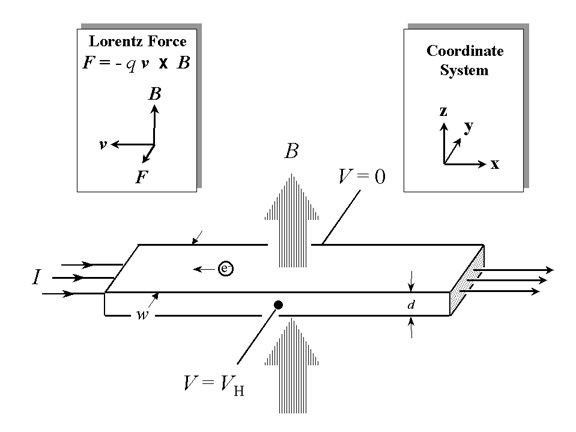
\includegraphics[width = 90mm]{fig1.jpg}
	\caption{Sýnimynd af mælingu á Hall-spennu, tekin af heimasíðu NIST. ($I$ er rafstraumur, $B$ er segulsvið og $V_H$ er Hall-spennan).}
	\label{fig:nist1}
\end{figure}

\section{Líkan}
Góð leið til þess að mæla Hall spennu í ferningslaga sýni er með því að láta straum renna eftir hornalínu þess og mæla síðan spennumuninn á hinum tveimur hornunum. Þessa uppstillingu má nota yfir öll horn sýnisins til að fá sem nákvæmastar niðurstöður. 

\begin{figure}[H]
\centering
	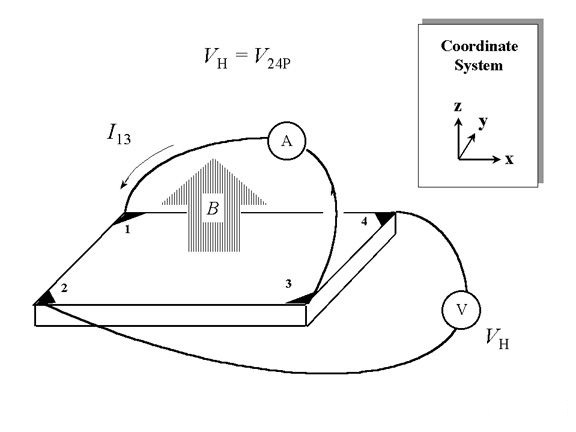
\includegraphics[width = 90mm]{fig3.jpg}
	\caption{Einföld sýnimynd af Hall-hrifum, tekin af heimasíðu NIST.}
	\label{fig:nist2}
\end{figure}

Út frá þessum mælingum má reikna þéttleika burðaragna straumsins með jöfnunni:

\begin{align}
n = \frac{IB}{qd|V_H|}
\end{align}

Hér er $q$ einingarhleðslan og $d$ er þykkt sýnisins. Þetta má einfalda með því að gera ráð fyrir að þessi þéttleiki sé jafndreifður þvert í gegnum sýnið, en þá getum við skilgreint þéttleika hleðslubera á lengdareiningu sem:

\begin{align}
n_s = nd = \frac{IB}{q|V_H|}
\end{align}

Í framhaldi af þessu má nota þéttleikann til þess að reikna hreifanleika hleðsluberanna með jöfnunni:

\begin{align}
    \mu = \frac{d}{qn_s\rho} = \frac{1}{qn_sR_s}
\end{align}

En hér er $\rho$ eðlisviðnám sýnisins, og $R_s = \rho/d$ er skilgreint til samskonar einföldunar og $n_s$. Til þess að reikna hreyfanleikann þarf því að mæla þetta viðnám, en það má gera með hinni svokölluðu van der Pauw aðferð. Aðferðin felst í því að mæla spennu og straum yfir aðliggjandi horn sýnisins og reikna út frá þeim mælingum viðnámin $R_A$ og $R_B$, þ.e. langsum og þversum um sýnið.

\begin{figure}[H]
\centering
	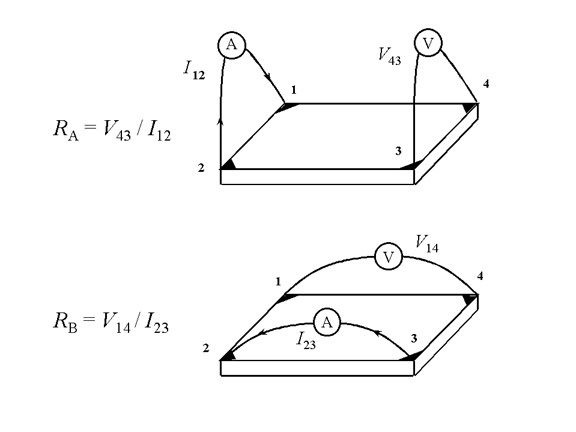
\includegraphics[width = 90mm]{fig2.jpg}
	\caption{Einföld sýnimynd af van der Pauw mælingum, tekin af heimasíðu NIST.}
	\label{fig:nist3}
\end{figure}

Viðnámin $R_A$ og $R_B$ tengjast síðan stærðinni $R_s$ með jöfnunni

\begin{align}
e^{-\pi \frac{R_A}{R_s}} + e^{-\pi \frac{R_B}{R_s}} = 1
\end{align}

Þessa jöfnu má leysa tölulega fyrir $R_s$.\\
\\
Nú geta burðaragnir straumsins í efninu okkar verið annaðhvort rafeindir eða holur, þ.e. efnið getur verið $n$-leiðandi eða $p$-leiðandi. Einfalt er að sjá hvort tilfellið á við út frá uppstillingu mælinga. Af mynd \ref{fig:nist2} sjáum við að formerki mældu Hall-spennunar fer eftir hleðslu burðaragna straumsins. Ef rafstraumurinn rennur úr horni $1$ yfir í horn $3$, þá verður þéttleiki hleðslubera mun hærri nær horni $2$ en horni $4$ vegna Lorentz kraftsins. Ef Hallspennan er mæld $V_H = V_{24} = V_2 - V_4$ þá sjáum við að ef við fáum $V_H > 0$ þá er $V_2 > V_4$, en það þýðir að hleðsluberarnir hafa jákvæða rafhleðslu, þ.e. efnið er $p$-leiðandi. \\
\\
Eftir að tegund hleðsluberanna hefur verið ákvörðuð má áætla virkjunarorku íbóta, $E_A$, þ.e. orkubilið á milli Fermi-orku efnisins, $E_F$, og leiðniborðans, $E_C$ (fyrir $n$-leiðara), eða gildisborðans, $E_V$ (fyrir $p$-leiðara). 

\begin{figure}[H]
\centering
	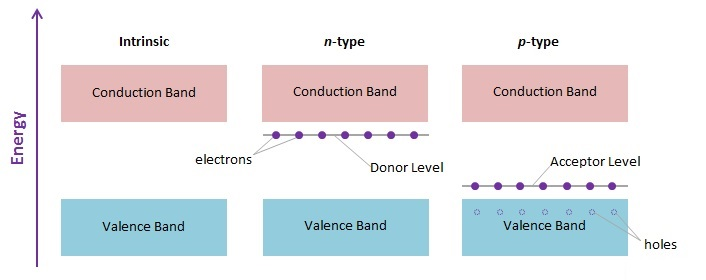
\includegraphics[width = 130mm]{nptype.jpg}
	\caption{Sýnimynd af orkugeil: a) Eiginleiðandi efni, b) $n$-leiðandi efni og c) $p$-leiðandi efni.}
	\label{fig:Bandgap}
\end{figure}

Fyrir lág hitastig má tengja þéttleika burðaragnanna við þessa virkjunarorku með jöfnunum:

\begin{align}
\frac{n_s}{d} = n_0 &= N_C e^{-(E_C-E_F)/k_BT}\nonumber\\
    & = N_C e^{-E_A/k_BT}
\end{align}

fyrir $n$-leiðara, og:

\begin{align}
\frac{n_s}{d} = p_0 &= N_V e^{-(E_F-E_V)/k_BT}\nonumber\\
    & = N_V e^{-E_A/k_BT}
\end{align}

fyrir $p$-leiðara. Þá sést að $\ln(n_s) = C - \frac{E_A}{k_B T}$, þar sem $C$ er einhver fasti. Graf af $\ln(n_s)$ sem fall af $1/k_BT$ ætti því að hafa hallatölu $-E_A$.

\newpage

\section{Framkvæmd}
Ferningslaga Si sýni af þykkt $d = \SI{525e-6}{m}$, dópað með óþekktu efni, var tengt við straum- og spennumæla á hornunum eins og rætt var í líkaninu hér að ofan. Sýninu var síðan komið fyrir ofan við mjög öflugan segul í kerfi sem kælt var niður í $\SI{23}{K}$ og fastur straumur látinn renna í gegnum það. Segulsviðið var látið færast úr $\SI{0.6}{T}$ niður í $\SI{-0.6}{T}$ í $\SI{0.2}{T}$ skrefum og í hverju skrefi voru framkvæmdar mælingar. Þetta var síðan endurtekið fyrir hærri og hærri hitastig upp að $\SI{300}{K}$. Í upphafi voru aðeins tekin hitastigs-skref upp á $\SI{1}{K}$ þar sem viðnám sýnisins breyttist mikið við lág hitastig, og reglulega þurfti að stilla af rafstrauminn, en við hærri hitastig voru skrefin hækkuð í $\SI{5}{K}$ og loks $\SI{10}{K}$.

\section{Niðurstöður}
Formerki á mældri Hall-spennu miðað við formerki á straum og segulsviði gefur til kynna að sýnið okkar sé $p$-leiðandi. Tekið var mark á legu sýnis með tilliti til segulsviðs.
\begin{figure}[H]
    \centering
    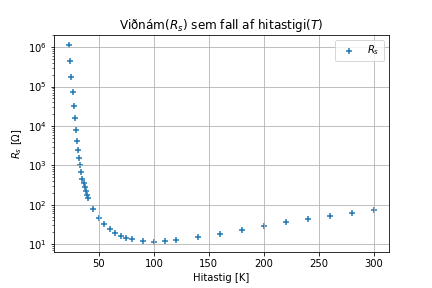
\includegraphics{R_s.PNG}
    \caption{Reiknuð gildi á $R_s$ út frá mælingum sem fall af hitastigi}
    \label{fig:R_s}
\end{figure}

Viðnám fellur með hitastigi eins og búast má við fyrir hálfleiðara en byrjar síðan að aukast hægt vegna aukinnar hljóðeinda-dreifingu.

\begin{figure}[H]
    \centering
    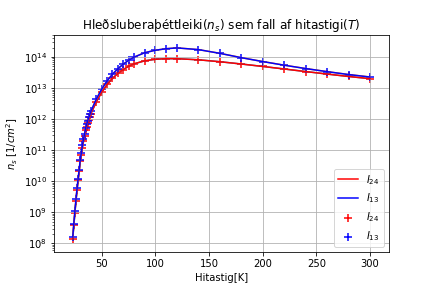
\includegraphics{n_s.PNG}
    \caption{Reiknuð gildi á $n_s$ sem fall af hitastigi. Rauða línan fæst fyrir strauminn $I_{13}$ og sú gula fyrir $I_{24}$ m.v. mynd \ref{fig:nist2}.}
    \label{fig:n_s}
\end{figure}
Athugum að örlítill munur fæst á ferlunum eftir því hvort við mælum $I_{13}$ eða $I_{24}$ en það er við því að búast og kemur líkleg til vegna einhverrar lítillar ósamhverfu í efninu. 

Við sjáum einnig að hleðsluberaþéttleiki eykst hratt við lág hitastig en fer síðan aftur lækkandi þegar hitastigið hækkar. Þetta er í samræmi við hegðunina á viðnáminu($R_s$), þar sem $n_s\propto I \propto \frac{1}{R}$.


\begin{figure}[H]
    \centering
    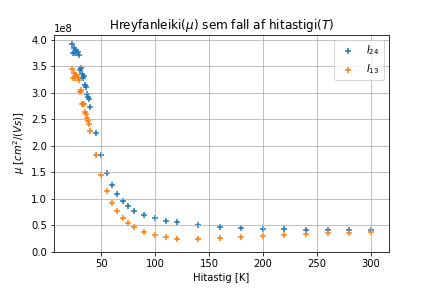
\includegraphics{mu.PNG}
    \caption{Reiknuð gildi á $\mu$ sem fall af hitastigi. Rauða línan fæst fyrir strauminn $I_{13}$ og sú gula fyrir $I_{24}$ m.v. mynd \ref{fig:nist2}.}
    \label{fig:mu}
\end{figure}

Við sjáum aftur tvenns konar ferla þar sem hreyfanleiki í stefnu $I_{13}$ er lægri en hreyfanleiki í stefnu $I_{24}$. Þetta er einnig í samræmi við hegðun viðnámsins $R_s$.

\begin{figure}[H]
    \centering
    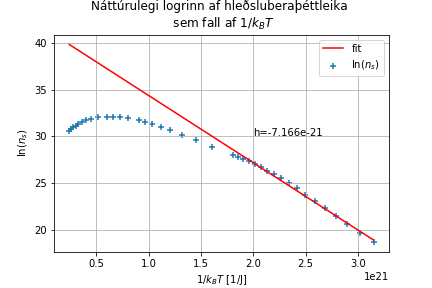
\includegraphics{nl(n_s).PNG}
    \caption{Lína (gul) er mátuð við gögnin (blá) við lág hitastig,\\ Hallatala línu svarar til $-E_A$}
    \label{fig:ln(n_s)}
\end{figure}

Út frá hallatölu á mynd \ref{fig:ln(n_s)} getum við áætlað virkjunarorku íbótar($E_A$) við lág hitastig og fáum að $E_A = \SI{7.163e-21}{J} = \SI{0.0447}{eV}$. Athugum að orkugeil Si er $E_{g}(T=\SI{0}{K}) = \SI{1.17}{eV}$ og $E_{g}(T=\SI{300}{K}) = \SI{1.11}{eV}$ svo $E_A\approx0.04E_{g}$. Fræðin segja okkur svo að við há hitastig má búast við $E_A = \frac{E_g}{2}$.\\


Niðurstöður mælinga okkar er í samræmi við líkan og rennir stoðum undir þau fræði sem þau byggjast á. Það er örlítið misræmi á mælingum eftir á milli hvaða horna á sýninu er mælt en það má útskýra því sýnið er ekki fullkomið. 



\end{document}
